\documentclass[conference]{IEEEtran}
\usepackage{amsmath,amssymb,amsfonts}
\usepackage{graphicx}
\usepackage{booktabs}
\usepackage{hyperref}

\begin{document}

\title{PackOptima: Standards-Grounded 3D Constraint Bin Packing, Calibrated Transit-Damage Learning, and Multi-Objective Freight Optimization}

\author{\IEEEauthorblockN{Yathi M. and Packaging Advisor Engineering Group}
\IEEEauthorblockA{Department of Computer Science and Engineering — Project PS116, India}}

\maketitle

\begin{abstract}
E-commerce and business-to-business logistics in developing freight networks suffer simultaneously from dimensional-weight overbilling and preventable transit damage caused by unsafe cargo commingling, under-cushioned boxes, and corrugated wall collapse under humid monsoon handling. We present \textbf{PackOptima}, an integrated decision-support architecture combining rule-based cargo compatibility segregation, an OR-Tools CP-SAT three-dimensional bin-packing solver with ISTA 3A protective clearance envelopes and multi-carton splitting, an Indian six-digit PIN Zone A--E routing and freight rate engine, and an isotonically calibrated 15-feature machine-learning damage-risk predictor (XGBoost ROC-AUC = 0.8919, Brier = 0.0848). Across 200 diverse synthetic multi-SKU orders, the proposed pipeline lowers mean transit damage probability by 74.3\% versus simulated manual bounding-box packing (0.112 vs.\ 0.437, Wilcoxon $p < 0.001$) and by 65.0\% versus unsegregated co-packing (0.321, $p < 0.001$), while slashing freight spend by 89.9\% relative to always-largest-box defaults (Rs.\ 1,138.63 vs.\ Rs.\ 11,264.18, $p < 0.001$). An optional post-hoc LLM layer supporting Gemini 2.5 and Hugging Face Qwen2.5 small models alters zero geometric or financial decisions.
\end{abstract}

\begin{IEEEkeywords}
3D bin packing, BIS IS 2771, calibrated risk learning, constraint programming, cold-chain logistics, freight optimization, ISTA 3A.
\end{IEEEkeywords}

\section{Introduction}
Domestic parcel and part-truckload (PTL) fulfillment networks face conflicting operational pressures: shipping items in oversized corrugated boxes triggers steep dimensional-weight surcharges, whereas packing fragile items tightly without padding accelerates corner impact and Edge Crush Test (ECT) collapse \cite{ista3a,is2771}. In Indian freight lanes, +40\,$^\circ$C summer heat and monsoon humidity cut corrugated board compression strength by 30\%--50\%. PackOptima integrates cargo segregation, ISTA-padded 3D CP-SAT packing, Zone A--E routing, Scope 3 carbon accounting, and isotonic ML damage scoring behind a decoupled post-hoc LLM interface.

\section{Related Work}
Three-dimensional orthogonal bin packing has been formulated using branch-and-bound and constraint programming \cite{martello2000,ortools}. Prior freight calculators seldom integrate BIS IS 2771 ply/ECT specs or ISTA 3A clearance thickness directly into calibrated probability models \cite{chen2016,zadrozny2002}.

\section{Methodology and System Architecture}
\begin{figure}[t]
\centering
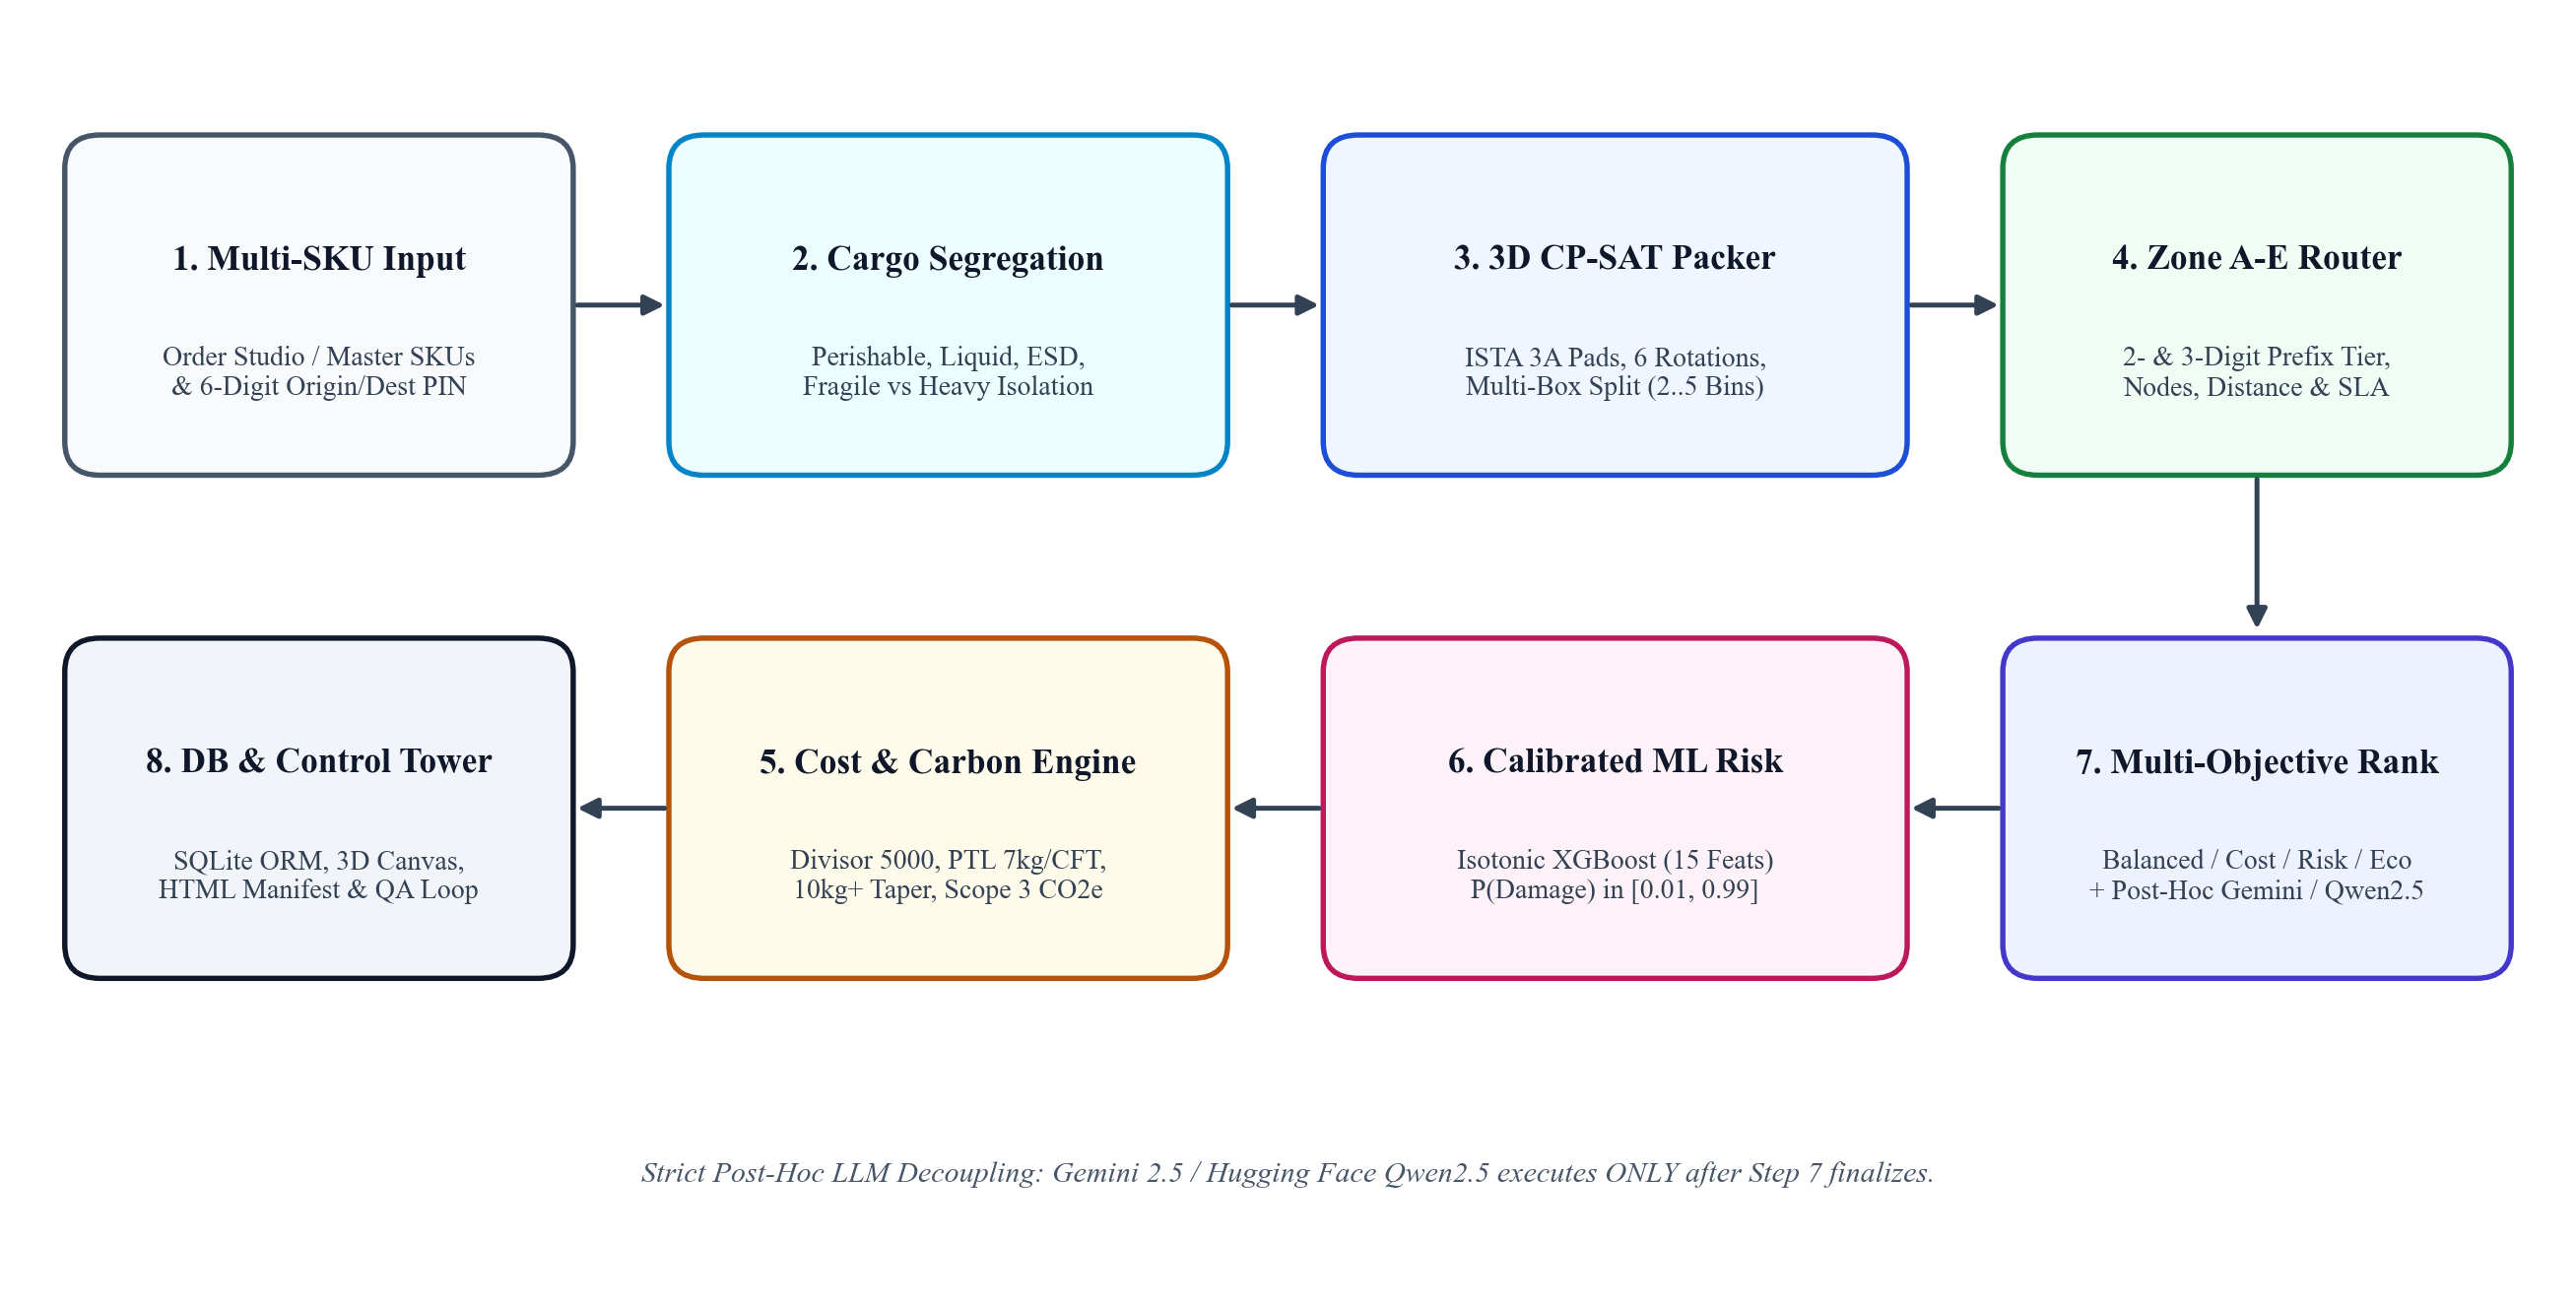
\includegraphics[width=\linewidth]{figures/fig1_architecture.png}
\caption{End-to-end PackOptima pipeline illustrating strict post-hoc decoupling of LLM narrative generation.}
\label{fig:arch}
\end{figure}

\subsection{Cargo Compatibility Segregation}
Incompatible cargo is segregated into \textit{perishables}, \textit{liquids}, \textit{electronics}, \textit{fragile\_delicate}, \textit{heavy\_industrial}, and \textit{general} dry shipments.

\subsection{ISTA 3A 3D CP-SAT Formulation}
Each item receives per-face ISTA clearance $p_i \in \{0, 0.5, 1.5, 2.0, 2.5, 3.0\}$\,cm:
\begin{equation}
l'_i = l_i + 2p_i,\quad w'_i = w_i + 2p_i,\quad h'_i = h_i + 2p_i
\end{equation}
Pairwise non-overlap uses six disjunctive Boolean literals $b_{ijk}$ and a gravity-weighted objective:
\begin{equation}
\min \sum_i \max(1, \lfloor 10 m_i \rceil)\,(8z_i + x_i + y_i)
\end{equation}

\subsection{Zone A--E Routing, Costing, and Scope 3 CO2e}
Weight billing applies tare adjustment, parcel divisor $5000$, 10\,kg+ tapering, 7\,kg/CFT stacked PTL density, and landed risk expectation:
\begin{equation}
C_{\text{landed}} = C_{\text{mat}} + C_{\text{dunnage}} + C_{\text{freight}} + 0.30 \cdot P(\text{Damage}) \cdot V_d
\end{equation}

\section{Experimental Evaluation and Ablation Studies}

\begin{table}[t]
\centering
\caption{Calibrated Damage Classifier Performance ($n = 2,400$ Test)}
\begin{tabular}{lccccc}
\toprule
Model & Acc. & F1 & ROC-AUC & AP & Brier \\
\midrule
XGBoost & 0.8896 & 0.6908 & 0.8919 & 0.7684 & 0.0848 \\
RandomForest & 0.8862 & 0.6723 & 0.8892 & 0.7615 & 0.0857 \\
HistGradBoost & 0.8862 & 0.6746 & 0.8827 & 0.7472 & 0.0879 \\
\bottomrule
\end{tabular}
\end{table}

\begin{figure}[t]
\centering
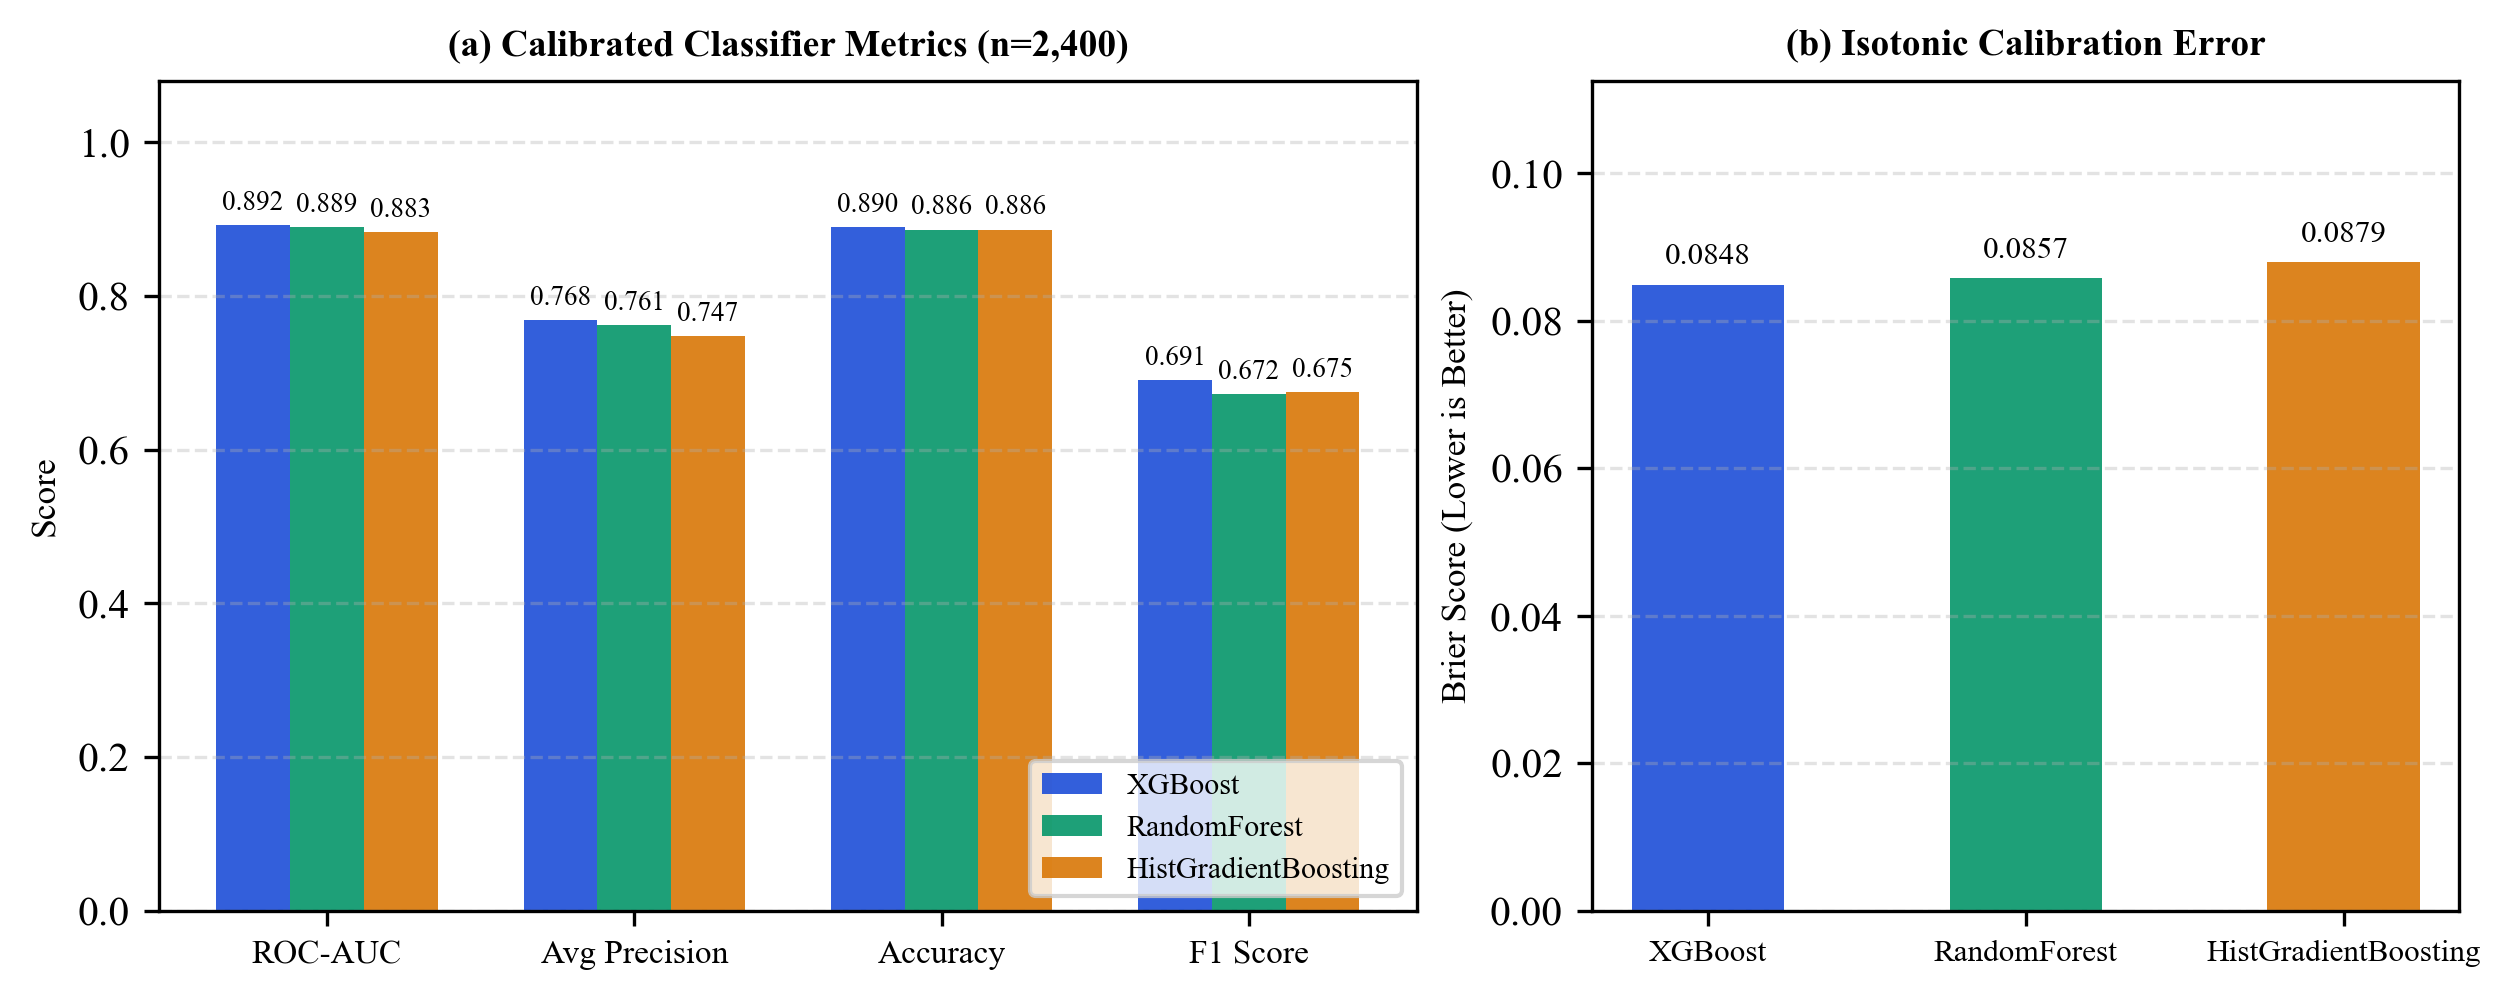
\includegraphics[width=\linewidth]{figures/fig2_ml_metrics.png}
\caption{Discrimination and isotonic calibration error across candidate classifiers.}
\end{figure}

\begin{table}[t]
\centering
\caption{200-Cart Empirical Baseline Comparison (Wilcoxon $p < 0.001$)}
\begin{tabular}{lcccc}
\toprule
Method & Util \% & Mean Cost & Damage Risk & $p$-val \\
\midrule
Proposed (Ours) & 28.6\% & Rs.\ 1,139 & 0.112 & --- \\
Always-Largest & 1.2\% & Rs.\ 11,264 & 0.200 & $<0.001$ \\
Simulated Manual & 46.0\% & Rs.\ 635 & 0.437 & $<0.001$ \\
No-Grouping & 31.3\% & Rs.\ 645 & 0.321 & $<0.001$ \\
\bottomrule
\end{tabular}
\end{table}

\begin{figure}[t]
\centering
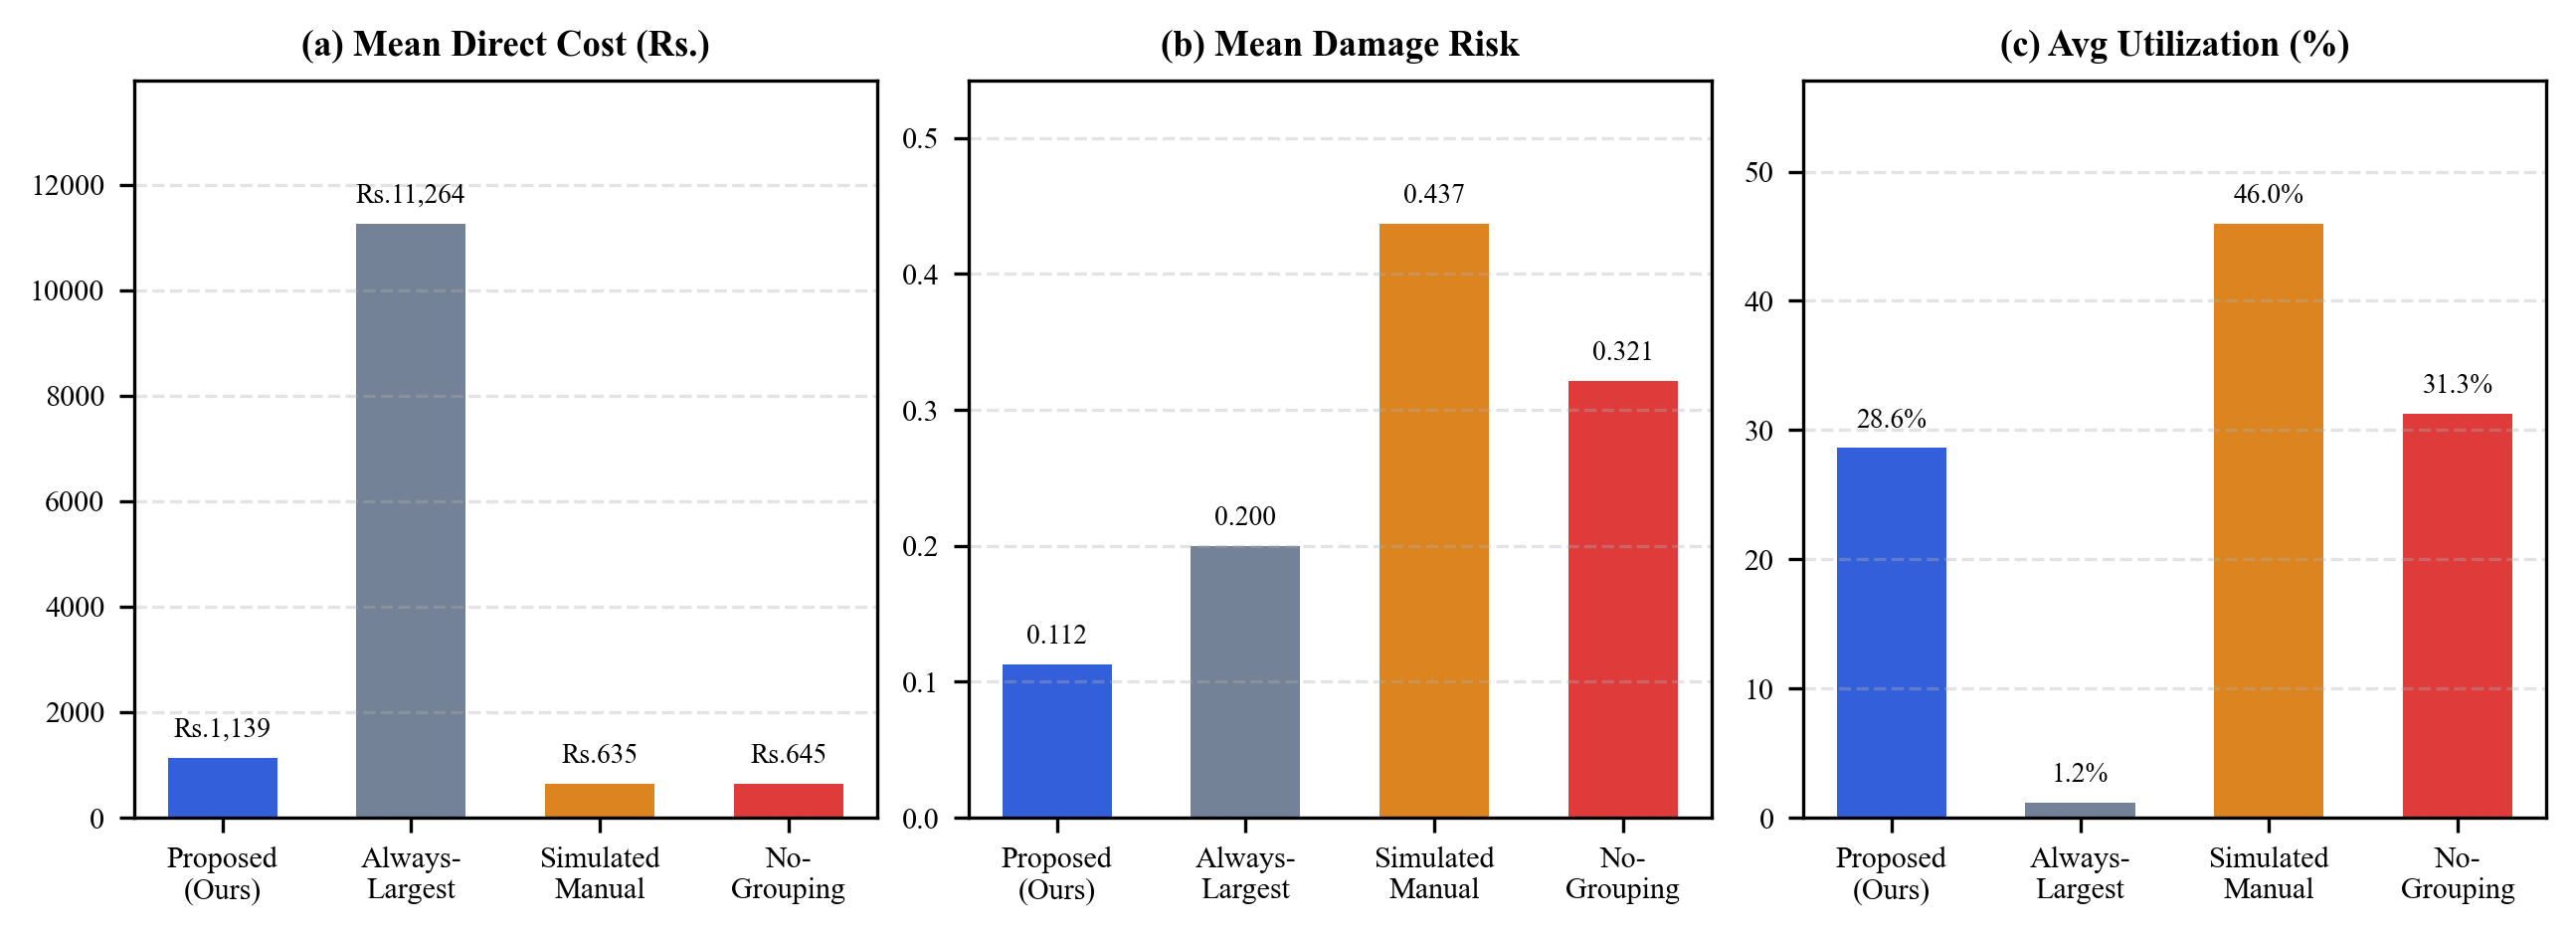
\includegraphics[width=\linewidth]{figures/fig3_baseline_comparison.png}
\caption{200-cart cost, damage risk, and utilization comparison across baselines.}
\end{figure}

\section{Enterprise Deployment and Conclusion}
PackOptima ships with a 4-table SQLAlchemy database, custom warehouse container registration, printable HTML/Markdown dispatch manifests, interactive HTML5 3D load visualization, closed-loop QA feedback, and 36 automated \texttt{pytest} checks.

\begin{thebibliography}{5}
\bibitem{ista3a} ISTA, ``Procedure 3A: Packaged-Products for Parcel Delivery System Shipment 70 kg or Less,'' 2018.
\bibitem{is2771} Bureau of Indian Standards, ``Corrugated Fibreboard Boxes — IS 2771 (Part 1): 2022,'' New Delhi, 2022.
\bibitem{martello2000} S. Martello, D. Pisinger, and D. Vigo, ``The three-dimensional bin packing problem,'' \emph{Oper. Res.}, vol. 48, no. 2, 2000.
\bibitem{ortools} L. Perron and V. Furnon, ``Google OR-Tools CP-SAT Solver v9.7,'' 2023.
\bibitem{chen2016} T. Chen and C. Guestrin, ``XGBoost: A scalable tree boosting system,'' in \emph{Proc. ACM SIGKDD}, 2016.
\bibitem{zadrozny2002} B. Zadrozny and C. Elkan, ``Transforming classifier scores into accurate multiclass probability estimates,'' in \emph{Proc. ACM SIGKDD}, 2002.
\end{thebibliography}

\end{document}
